\allowdisplaybreaks[4]
\section{Adaptive Noise Cancellation}
\subsection{Delay of ALE}
Due to the uncorrelation between interest signal and noise signal, the white noise can be eliminated by the delay version of the signal. The adaptive line enhancer (ALE) is used the delay of the noise-corrupted signal $s(n)$ to estimate the interest signal $\hat x(n)$. The optimal delay $\Delta$ can be calculated at the beginning of the Mean Squared Error.
\begin{align}
	\mathbb{E}\{(s(n)-\hat x(n))^2\}
	&=\mathbb{E}\{(x(n)+\eta(n)-\hat x(n))^2\}\notag\\
	&=\underbrace{\mathbb{E}\{\eta(n)^2\}}_{\eta^2}+\underbrace{\mathbb{E}\{(x(n)-\hat x(n))^2\}}_{\approx 0}+\underbrace{2\mathbb{E}\{(x(n)-\hat x(n))\eta(n)\}}_{minimize}
\end{align}
Therefore, for the optimal estimation, the MSE should be equal to the noise power. That is, only the last term should minimize.
\begin{align}
	\min_{\Delta} \mathbb{E}\left\{(x(n)-\hat x(n))\eta(n)\} \right\}
	&\Rightarrow \min_{\Delta} \mathbb{E}\left\{\hat x(n)\eta(n)\} \right \}\notag\\
	&=\min_{\Delta} \mathbb{E}\left\{v(n) + 0.5v(n-2)\mathbf w^T(n)\mathbf u(n)\right\}\notag\\
	&=\min_{\Delta} \mathbb{E}\left \{(v(n) + 0.5v(n-2))\sum_{i=0}^{M-1}\mathbf w^T(n)s(n-\Delta -i)\right\}\notag\\
	&=\min_{\Delta} \mathbb{E}\left \{(v(n) + 0.5v(n-2))\sum_{i=0}^{M-1}\mathbf w^T(n)(x(n-\Delta -i)+\eta(n-\Delta -i))\right\}
\end{align}
And due to uncorrelated of $x(n)$ and $v(n)$, equation above can be simplified to
\begin{align}
	&\min_{\Delta} \mathbb{E}\left \{(v(n) + 0.5v(n-2))\sum_{i=0}^{M-1}\mathbf w^T(n)(x(n-\Delta -i)+\eta(n-\Delta -i))\right\}\notag\\
	=&\min_{\Delta} \mathbb{E}\left \{(v(n) + 0.5v(n-2))\sum_{i=0}^{M-1}\mathbf w^T(n)\eta(n-\Delta -i)\right\}\notag\\
	=&\min_{\Delta} \mathbb{E}\left \{(v(n) + 0.5v(n-2))\sum_{i=0}^{M-1}\mathbf w^T(n)(v(n-\Delta -i)+v(n-\Delta-2 -i))\right\}\label{eq:MSe}\\
	\approx& 0 \to\Delta=2\notag
\end{align}
Therefore, observing Eq.\ref{eq:MSe}, the error will tend to zero only if the delay $\Delta$ is larger than 2. Since the time indexes of signal $v(n)$  are non-overlapping, resulting in uncorrelated. Fig.\ref{fig:2_3_a} depicts the effect of the delay $\Delta=1\sim4$ on the estimated signal $\hat x(n)$ with the fixed filter length $M=3$. The top row illustrated 100 realisations of $s(n)$, $\hat x(n)$, while the bottom row is the average signal of the estimation. When the delay $\Delta>3$, the noise signal (in yellow) is suppressed a lot, leading to a small MSE. Thus, the results prove the previous analysis.
\begin{figure}[htb]
    \centering
    \hspace{-0.4cm}
    \begin{subfigure}[b]{0.26\textwidth}
     \centering
     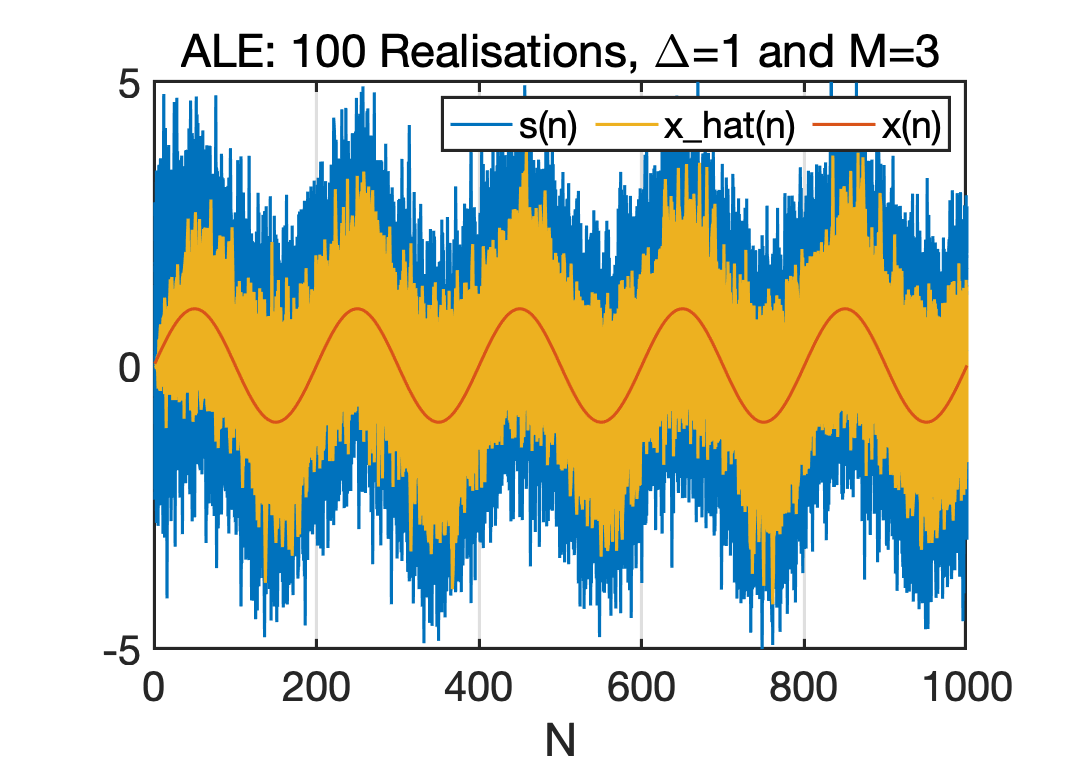
\includegraphics[width=\textwidth]{fig/23/23a1.eps}
    \end{subfigure}
    \hspace{-0.4cm}
    \begin{subfigure}[b]{0.26\textwidth}
     \centering
     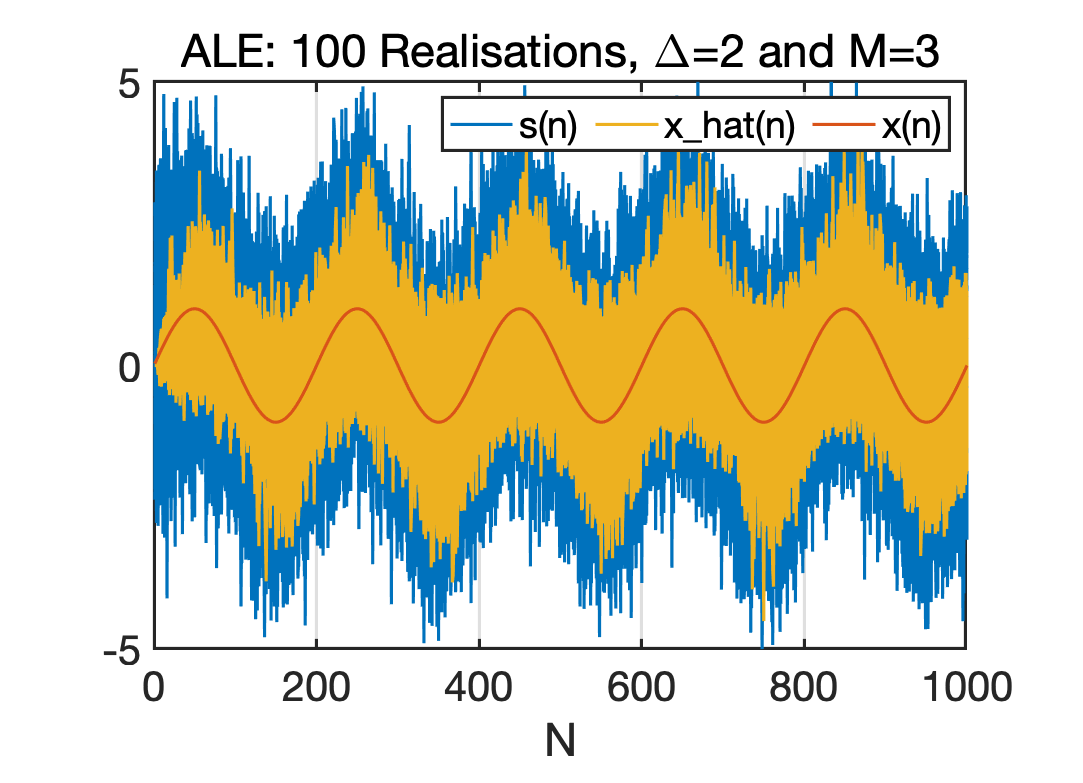
\includegraphics[width=\textwidth]{fig/23/23a3.eps}
    \end{subfigure} 
    \hspace{-0.4cm}
    \begin{subfigure}[b]{0.26\textwidth}
     \centering
     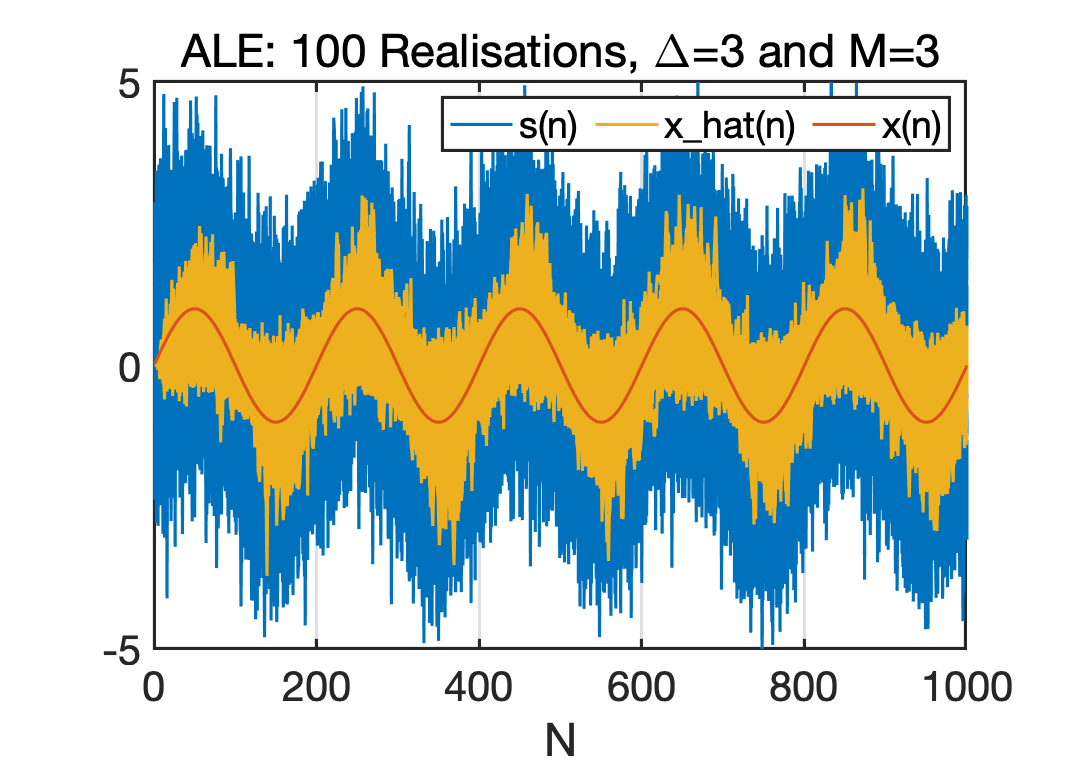
\includegraphics[width=\textwidth]{fig/23/23a5.eps}
    \end{subfigure}
    \hspace{-0.4cm}
    \begin{subfigure}[b]{0.26\textwidth}
     \centering
     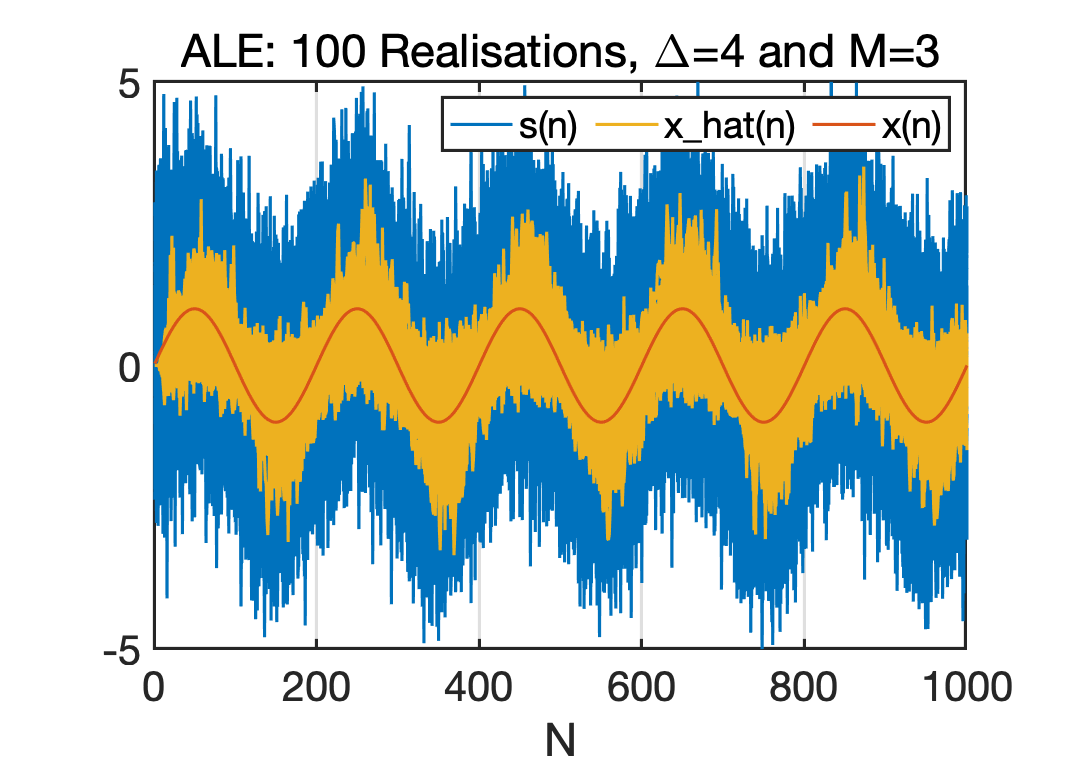
\includegraphics[width=\textwidth]{fig/23/23a7.eps}
    \end{subfigure}
    \\
    \hspace{-0.4cm}
    \begin{subfigure}[b]{0.26\textwidth}
     \centering
     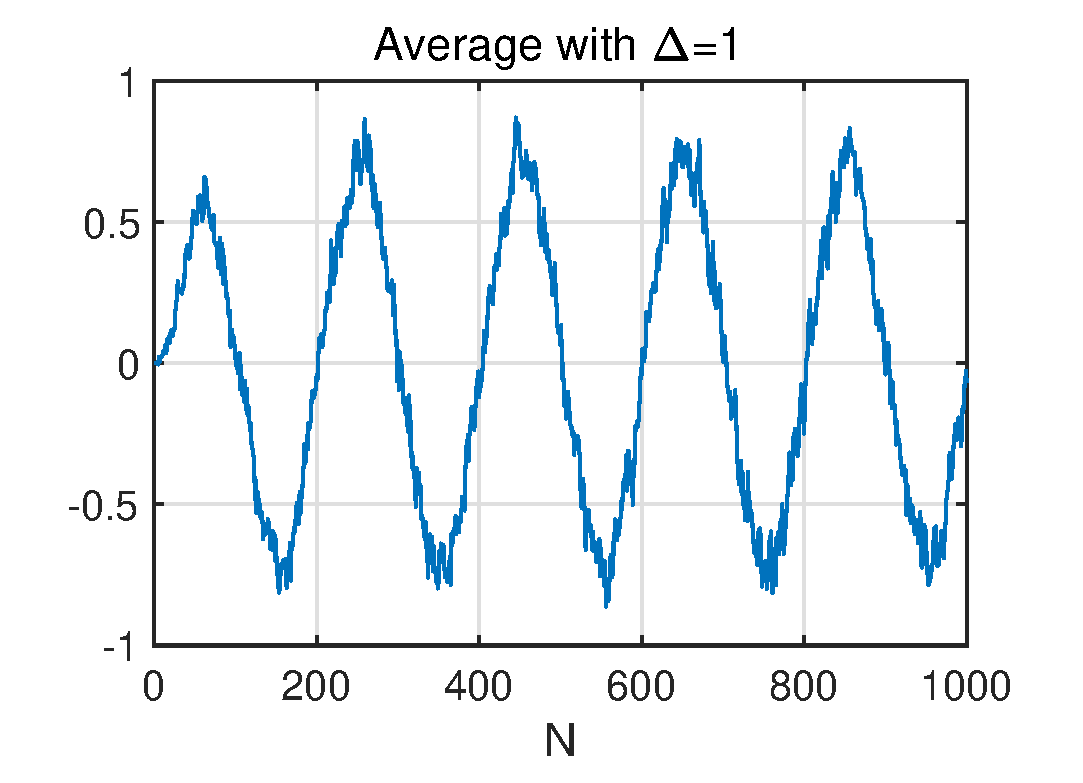
\includegraphics[width=\textwidth]{fig/23/23a2.eps}
    \end{subfigure}
    \hspace{-0.4cm}
    \begin{subfigure}[b]{0.26\textwidth}
     \centering
     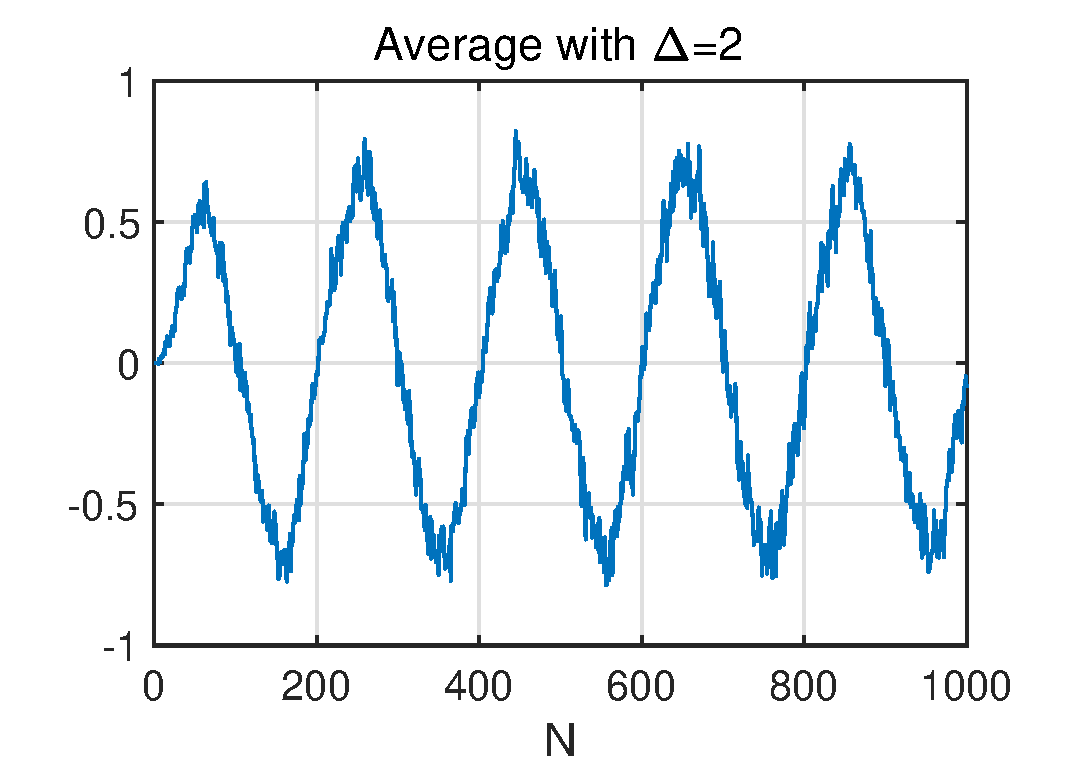
\includegraphics[width=\textwidth]{fig/23/23a4.eps}
    \end{subfigure} 
    \hspace{-0.4cm} 
    \begin{subfigure}[b]{0.26\textwidth}
     \centering
     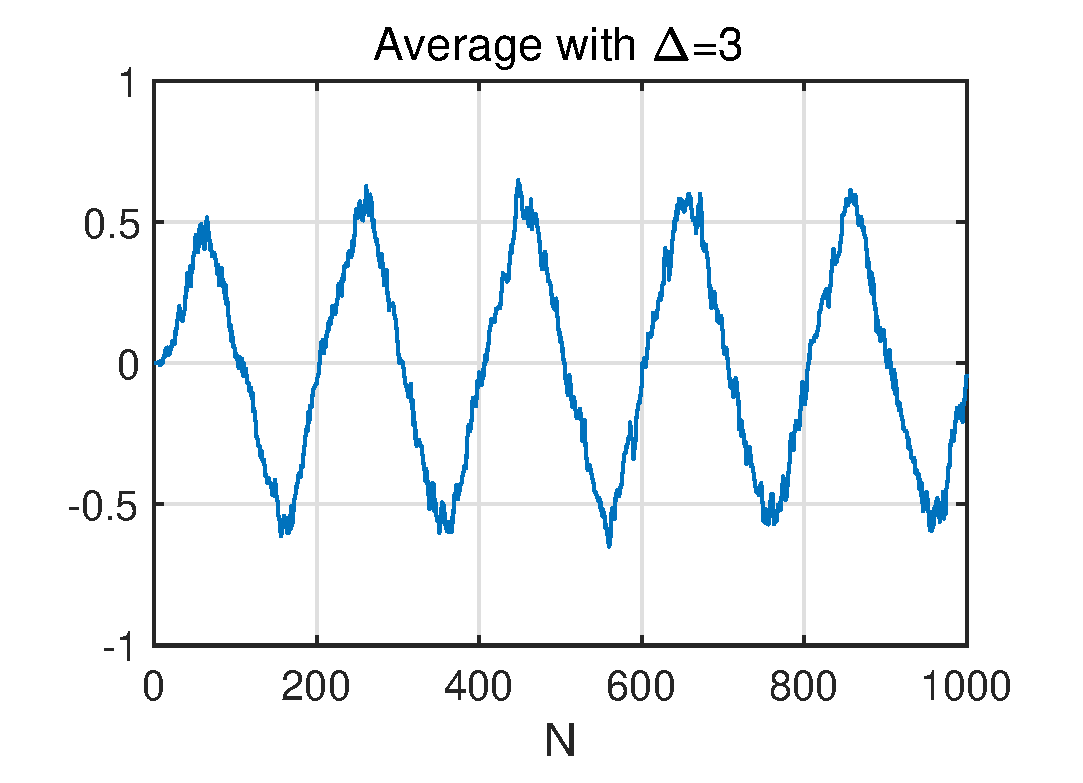
\includegraphics[width=\textwidth]{fig/23/23a6.eps}
    \end{subfigure}
    \hspace{-0.4cm}
    \begin{subfigure}[b]{0.26\textwidth}
     \centering
     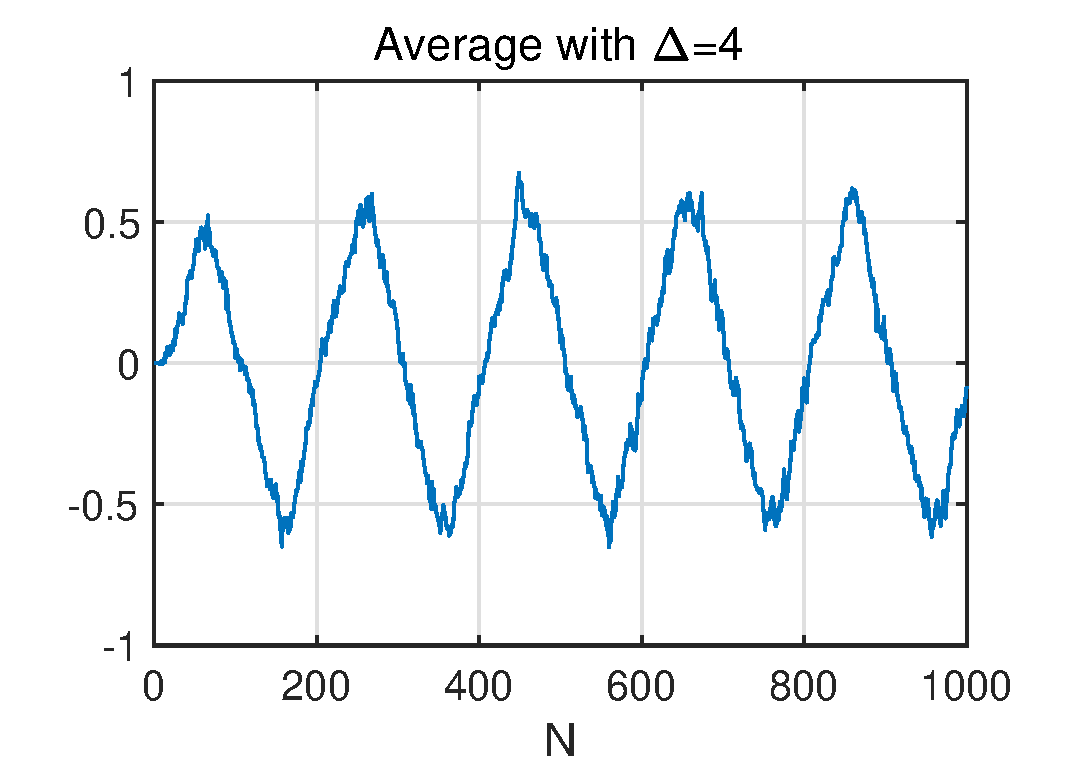
\includegraphics[width=\textwidth]{fig/23/23a8.eps}
    \end{subfigure}
    \caption{ALE: Effect of $\Delta$ with fixed $M=3$}
    \label{fig:2_3_a}
\end{figure}
\subsection{Effects of $M$ and delay on MSPE }
In order to find the optimal delay and the filter length $M$, this experiment calculates the MPSE by varying $\Delta$ from 1 to 25 and $M$ from 1 to 20. As shown in Fig.\ref{fig:2_3_b1}, neglecting the inappropriate values of $\Delta\leq 2$ and $M=1$, the MPSE curves both keep a increasing tendency with the growing of the delay and filter order. However, the MSPE remains approximately flat with a minimum error in range 3 to 6. When the filter order is large than 6, the over-modelling problem will occur, causing the growth of the MSPE. Notice that the performances of $\Delta=3$ and $\Delta=5$ are nearly same.
\begin{figure}[htb]
    \centering
    \hspace{-0.4cm}
    \begin{subfigure}[b]{0.4\textwidth}
     \centering
     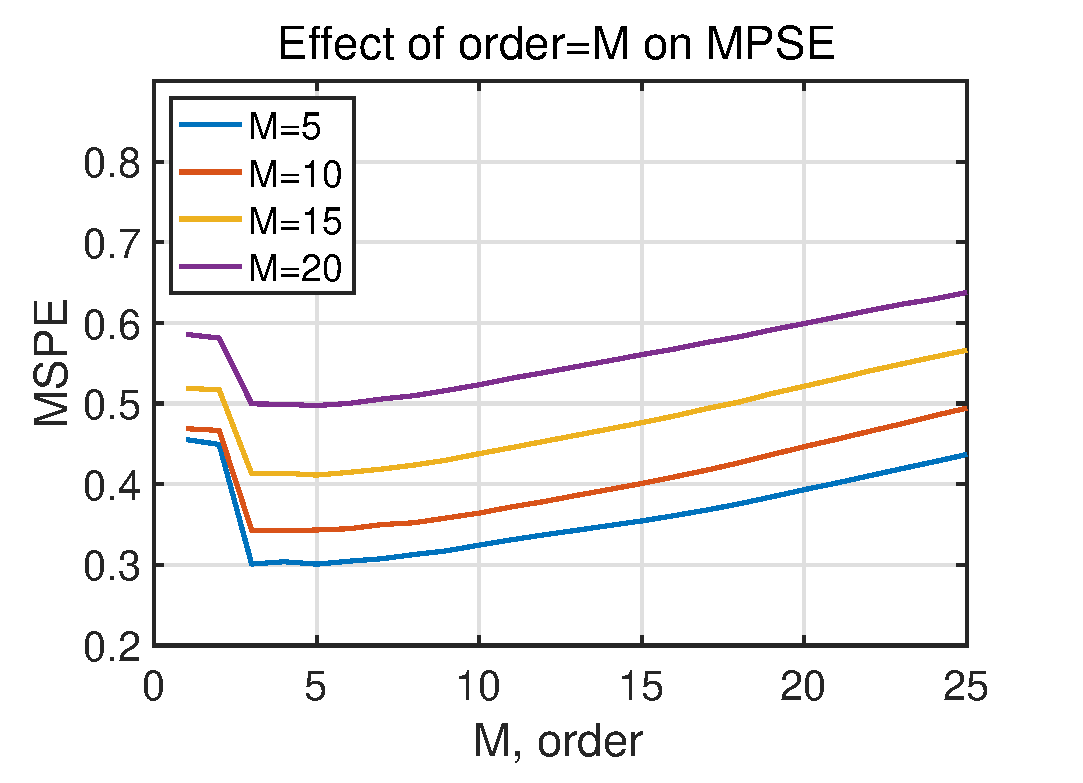
\includegraphics[width=\textwidth]{fig/23/23b2.eps}
    \end{subfigure}
    \hspace{1cm}
    \begin{subfigure}[b]{0.4\textwidth}
     \centering
     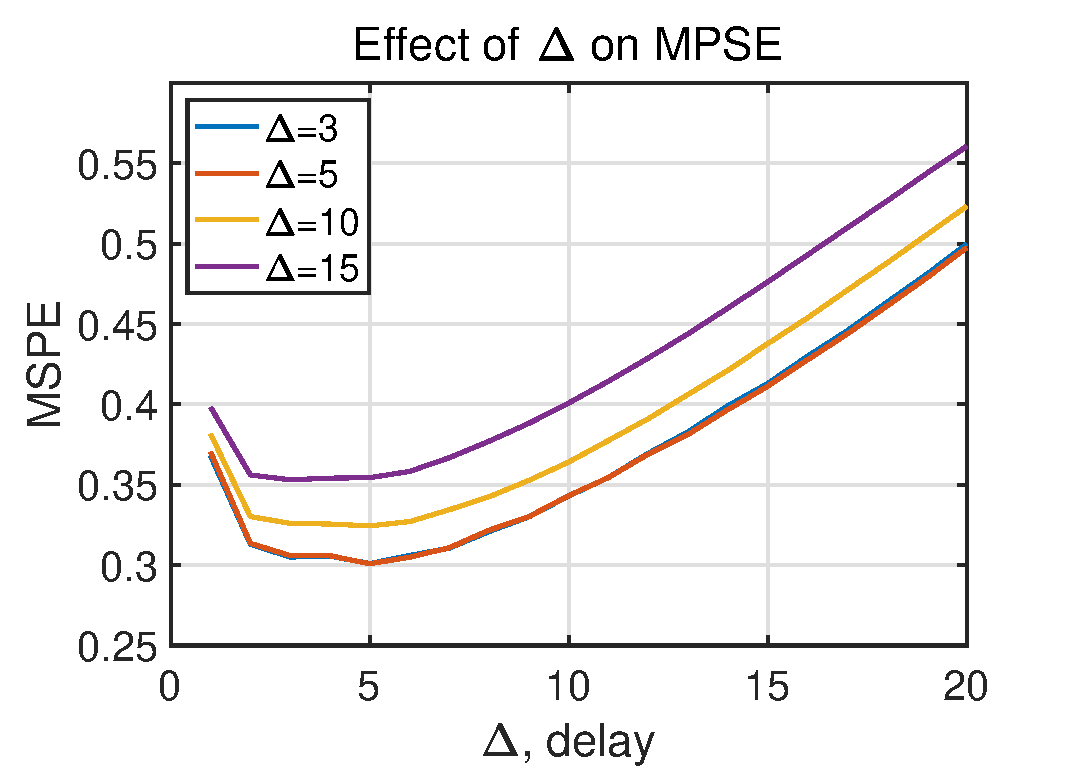
\includegraphics[width=\textwidth]{fig/23/23b1.eps}
    \end{subfigure} 
    \caption{ALE: Effect of $\Delta$ and $M$ on MSPE}
    \label{fig:2_3_b1}
\end{figure}\\
Observing the effect on varying delay, the MSPE curves approximately keep same in the range of $\Delta\in[3,6]$, which are similar as the ones of varying order $M$. Afterwards, the MSPE gradually rises up to the maximum when $\Delta=25$. If the delay is set to large, there is a lag between the estimated signal $\hat x(n)$ and actual signal $x(n)$, resulting in the increasing MSPE. As shown in Fig.\ref{fig:2_3_b2}, the realisations of optimal parameters ($M=3$, $\Delta=3$) and large delay ($M=3$, $\Delta=25$) are plotted. There is an obvious shift of estimated signal which proved the analysis. Due to the computational cost with increasing order, the relatively optimal parameters are $M=3$ and $\Delta=3$.
\begin{figure}[htb]
    \centering
    \hspace{-0.4cm}
    \begin{subfigure}[t]{0.37\textwidth}
     \centering
     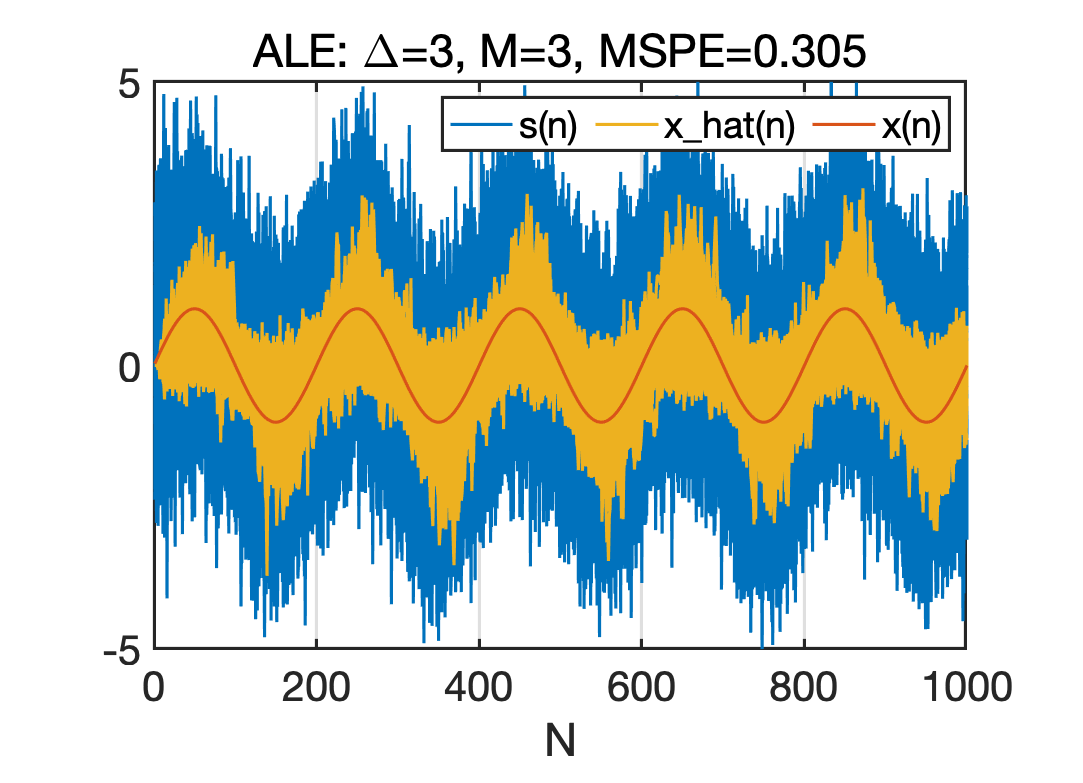
\includegraphics[width=\textwidth]{fig/23/23b3.eps}
    \end{subfigure}
    \hspace{0.4cm}
    \begin{subfigure}[t]{0.37\textwidth}
     \centering
     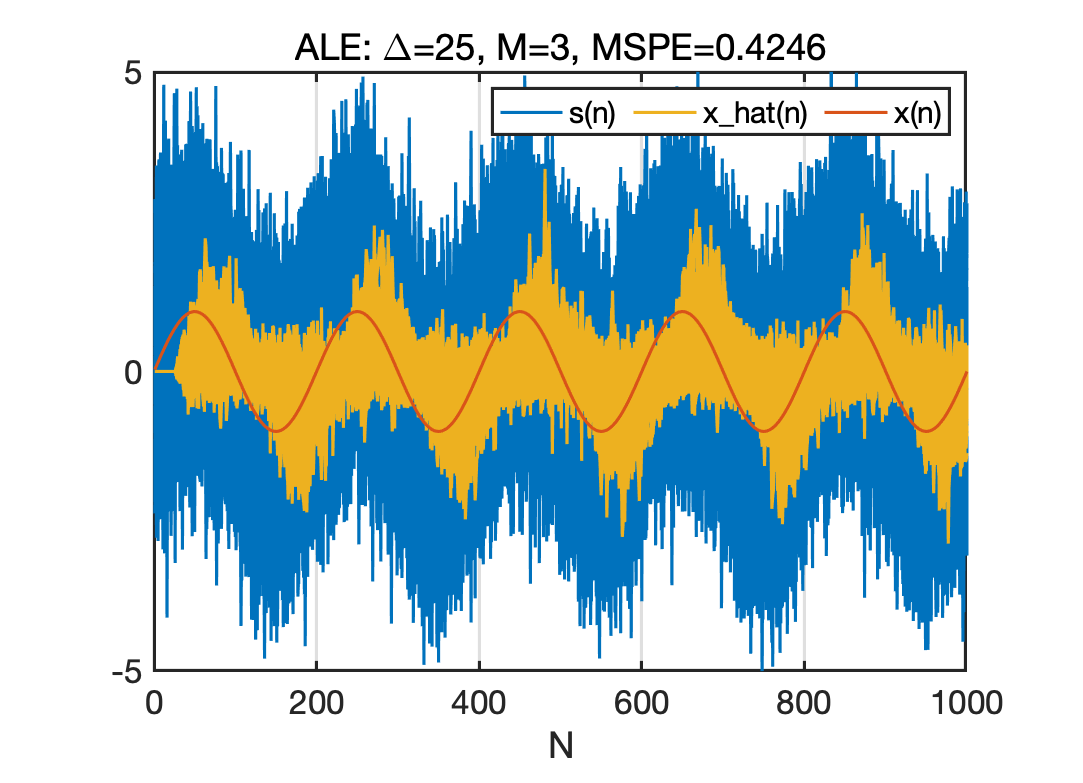
\includegraphics[width=\textwidth]{fig/23/23b4.eps}
    \end{subfigure} 
    \caption{ALE: Realisations of increasing $\Delta$ with fixed $M$}
    \label{fig:2_3_b2}
\end{figure}
\subsection{ANC vs ALE}
The adaptive noise cancellation (ANC) applied different input signal $\mathbf u(n)$ with correlated noise signal $\epsilon(n)$ whose aim is to estimate the noise $\eta(n)$. Thus, the desired signal $\hat x(n)$ is obtained by subtraction. The correlated secondary signal is assumed as $\epsilon(n) = 0.7\eta(n) + 0.01$. Fig.\ref{fig:2_3_c} illustrated the performance of ANC and ALE. At the beginning of the estimation, the noise is quite large. With the increasing of time index, the noise is almost eliminated. Therefore, the MSPE of ANC is 0.1098 which is approximately one third of the ALE. Observing the average plot, the ANC estimation is equal to the actual sine wave after 200 samples. Thus, the ANC has a high performance than the ALE.
\begin{figure}[htb]
    \centering
    \hspace{-0.4cm}
    \begin{subfigure}[b]{0.33\textwidth}
     \centering
     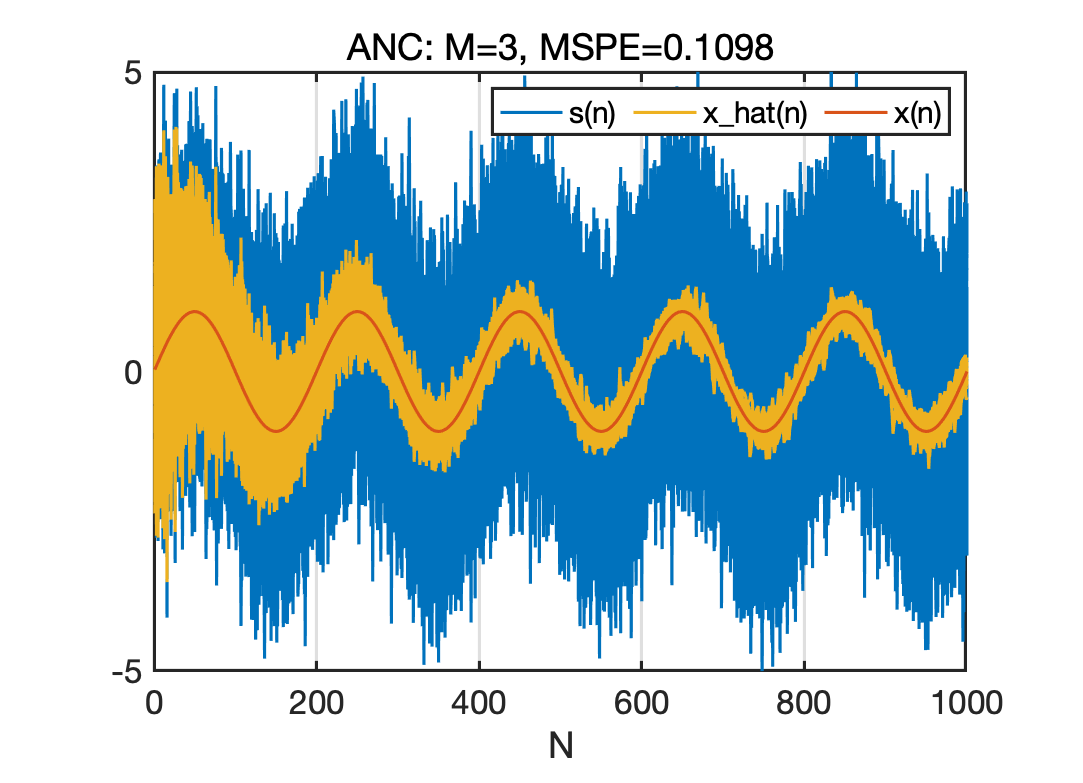
\includegraphics[width=1.1\textwidth]{fig/23/23c1.eps}
    \end{subfigure}
    \hspace{-0.1cm}
    \begin{subfigure}[b]{0.33\textwidth}
     \centering
     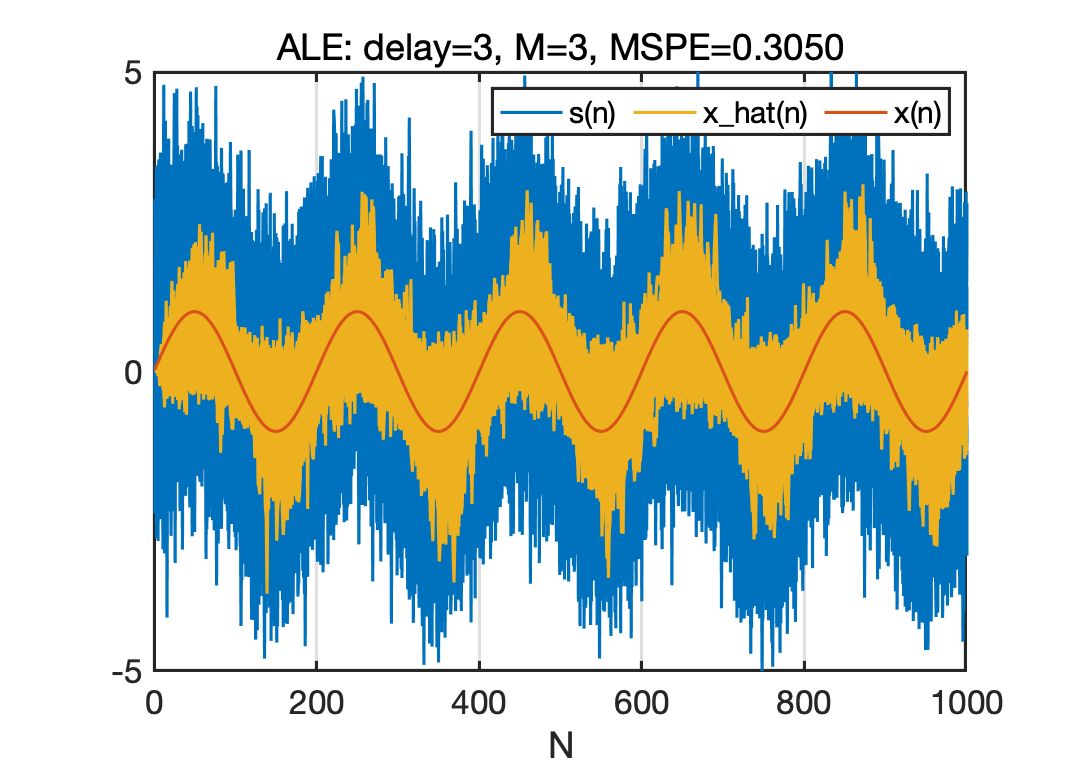
\includegraphics[width=1.1\textwidth]{fig/23/23c2.eps}
    \end{subfigure} 
    \hspace{-0.1cm}
    \begin{subfigure}[b]{0.33\textwidth}
     \centering
     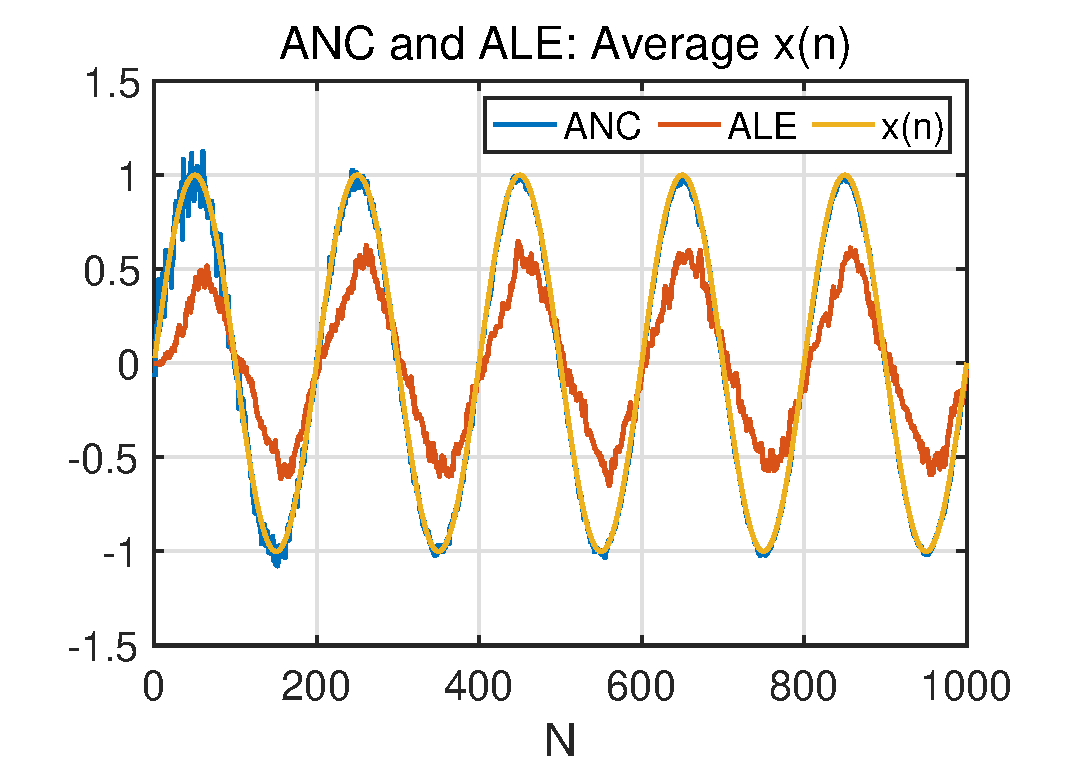
\includegraphics[width=1.1\textwidth]{fig/23/23c3.eps}
    \end{subfigure} 
    \caption{Performance of ANC and ALE}
    \label{fig:2_3_c}
\end{figure}
\subsection{ANC for EEG data}
In order to remove the strong component at $50Hz$, a noisy sine wave $\epsilon(n)$ with corresponding frequency is synthesised. Fig.\ref{fig:2_3_d1} shows the spectrogram of the original \texttt{POz} data with the rectangular window length of $2^{12}$ and 0.5 overlapping. There is an distinct line in yellow at $50Hz$ which should be removed.
\begin{figure}[htb]
    \centering
    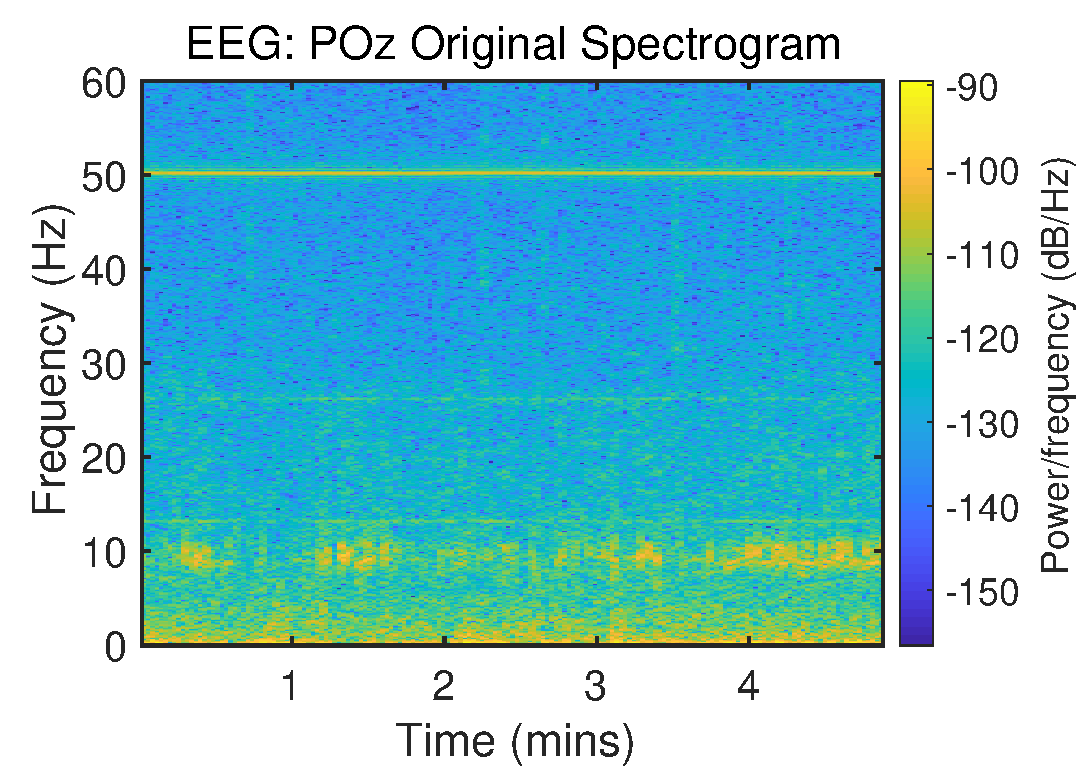
\includegraphics[width=0.35\textwidth]{fig/23/23d1.eps}
    \caption{EEG: Original Spectrogram}
    \label{fig:2_3_d1}
\end{figure}\\
Fig.\ref{fig:2_3_d2} shows the effects ANC by learning rate $\mu$ and $M$. When increasing the filter order $M$, the noisy component is getting to be removed more effectively. A under-modelling with small order causes residual of $50Hz$ component, while over-modelling results in excessively elimination. As to the $\mu$, large learning rate will affect the component around $50Hz$, leading to the attenuation of interest signal.
\begin{figure}[htb]
    \centering
    \hspace{-0.4cm}
    \begin{subfigure}[b]{0.32\textwidth}
     \centering
     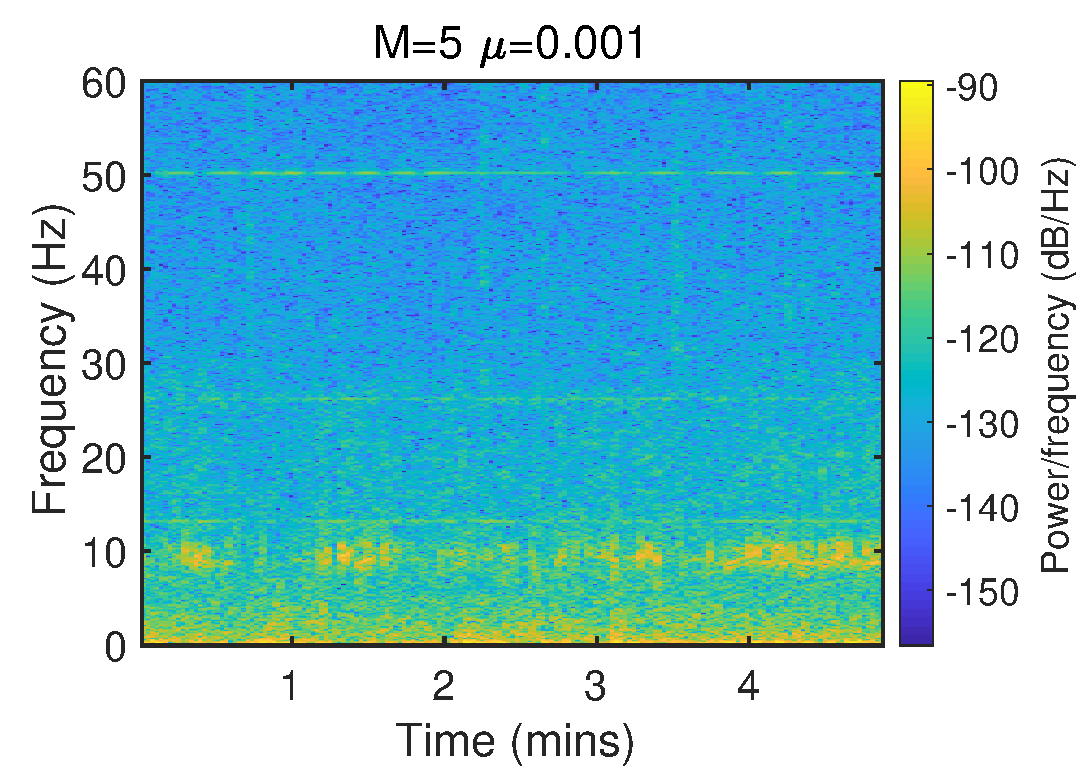
\includegraphics[width=\textwidth]{fig/23/23d2.eps}
    \end{subfigure}
    \hspace{-0.4cm}
    \begin{subfigure}[b]{0.32\textwidth}
     \centering
     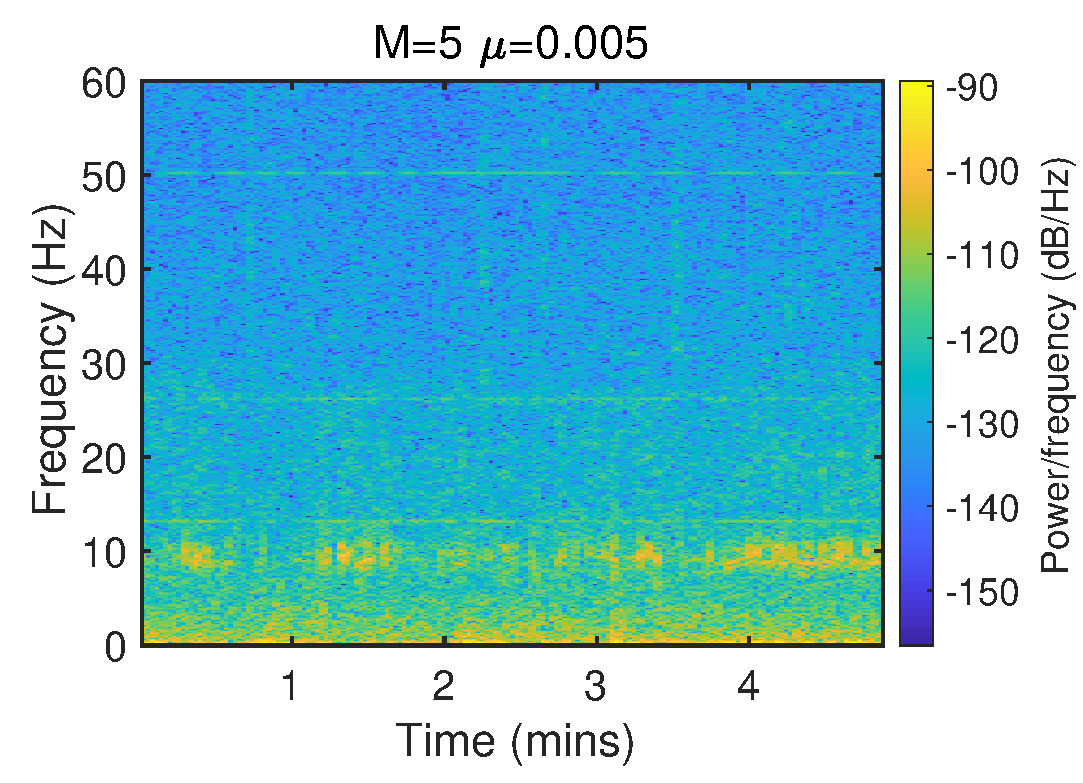
\includegraphics[width=\textwidth]{fig/23/23d3.eps}
    \end{subfigure} 
    \hspace{-0.4cm}
    \begin{subfigure}[b]{0.32\textwidth}
     \centering
     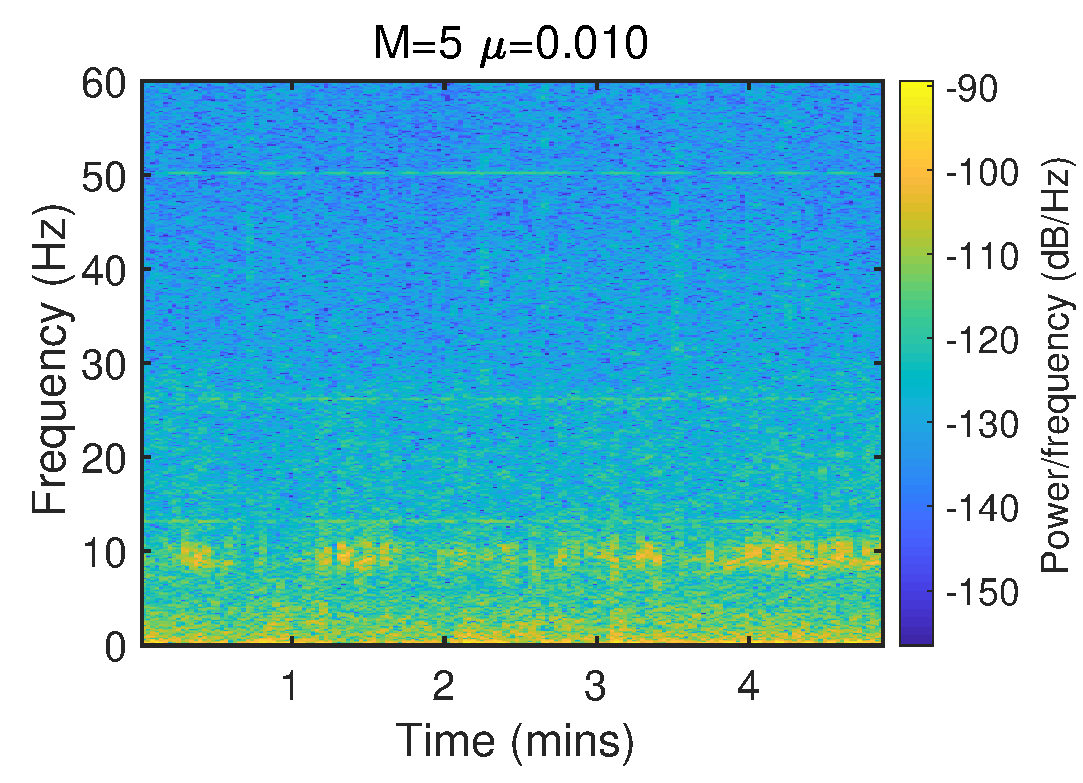
\includegraphics[width=\textwidth]{fig/23/23d4.eps}
    \end{subfigure}
    \\
    \hspace{-0.4cm}
    \begin{subfigure}[b]{0.32\textwidth}
     \centering
     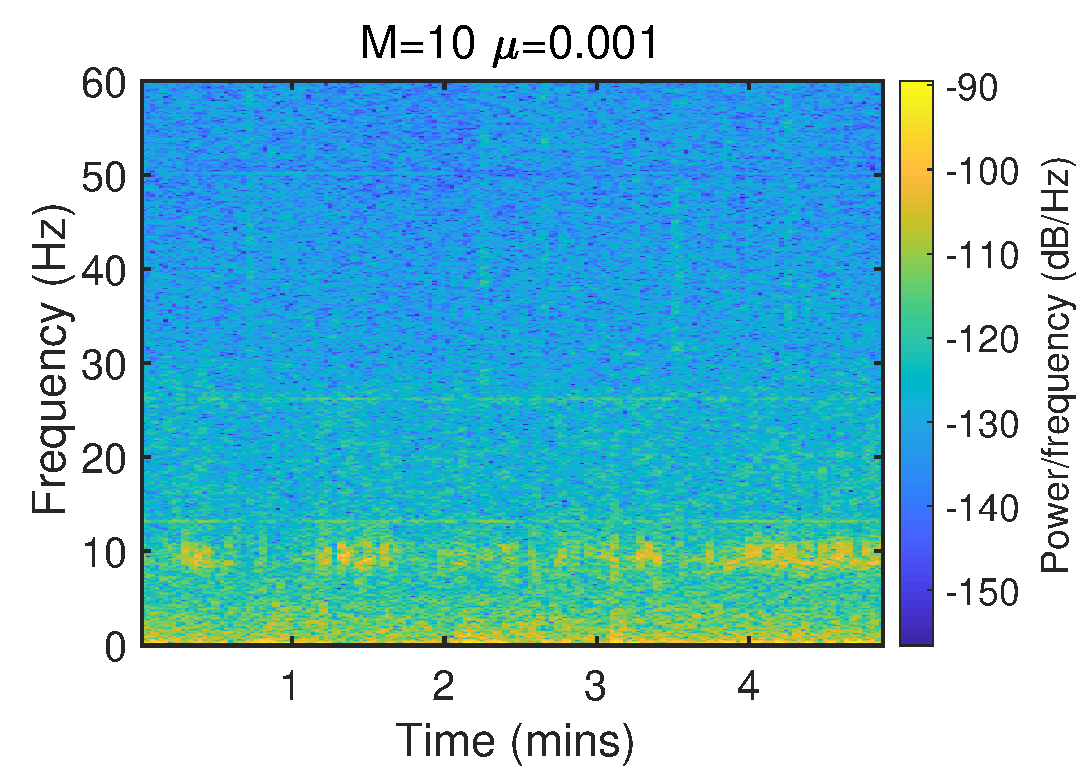
\includegraphics[width=\textwidth]{fig/23/23d5.eps}
    \end{subfigure}
    \hspace{-0.4cm}
    \begin{subfigure}[b]{0.32\textwidth}
     \centering
     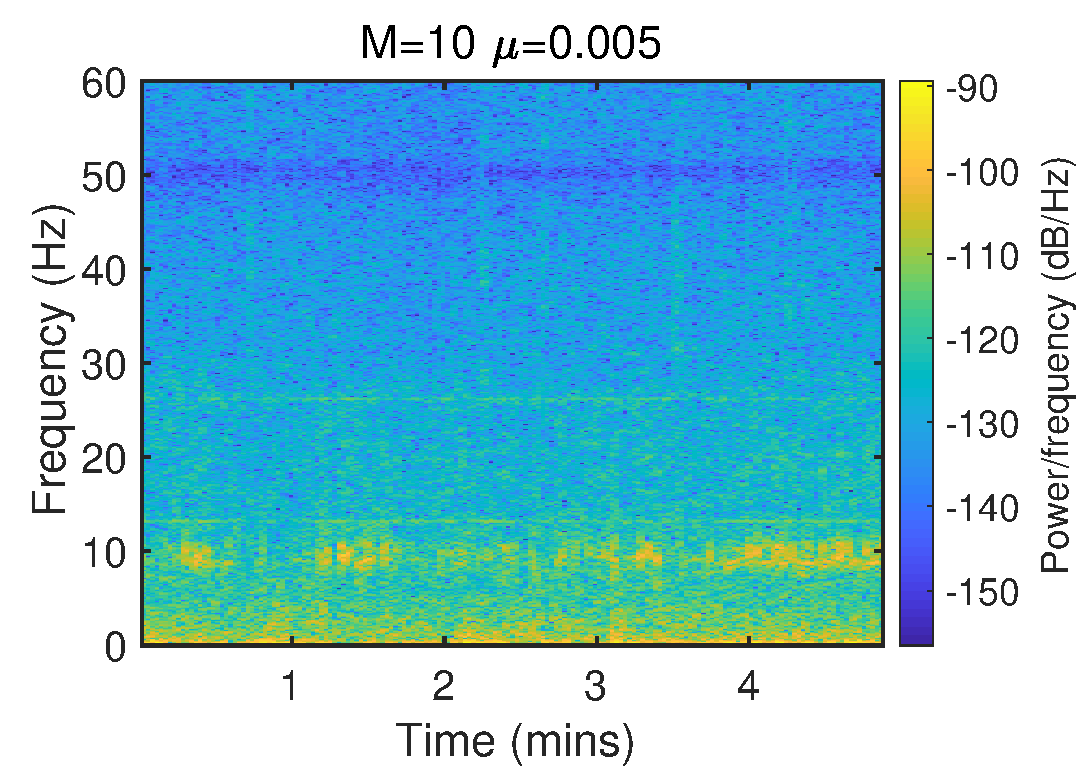
\includegraphics[width=\textwidth]{fig/23/23d6.eps}
    \end{subfigure}
    \hspace{-0.4cm}
    \begin{subfigure}[b]{0.32\textwidth}
     \centering
     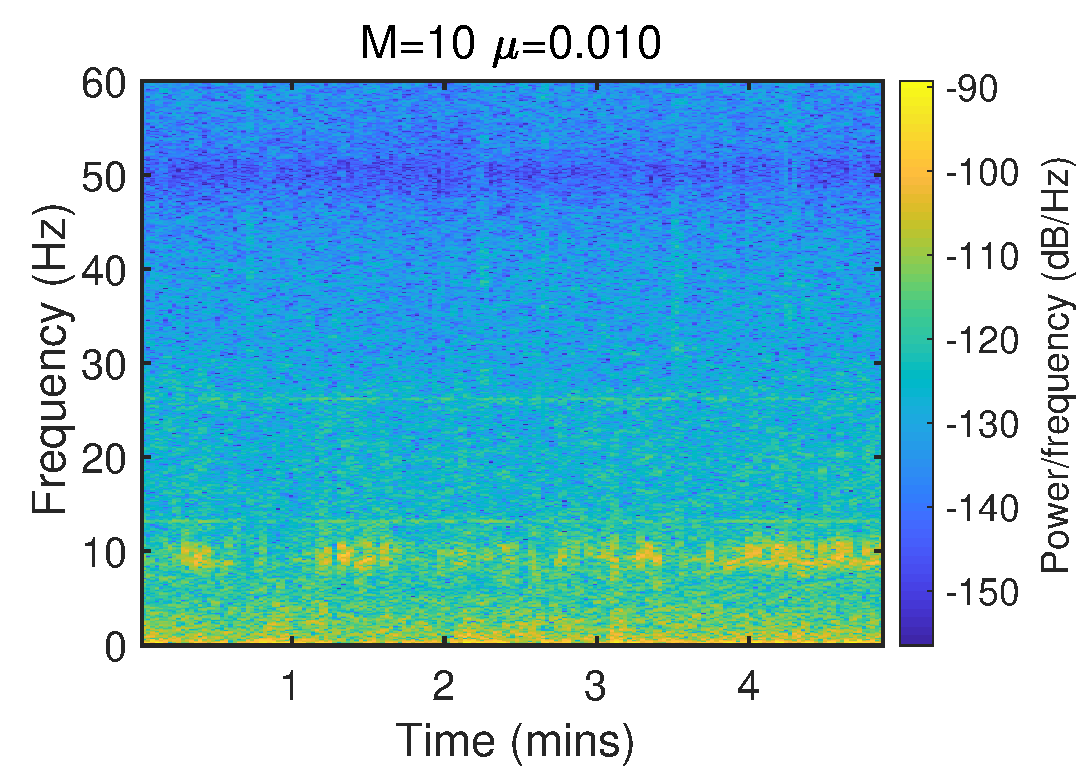
\includegraphics[width=\textwidth]{fig/23/23d7.eps}
    \end{subfigure}
    \\
    \hspace{-0.4cm} 
    \begin{subfigure}[b]{0.32\textwidth}
     \centering
     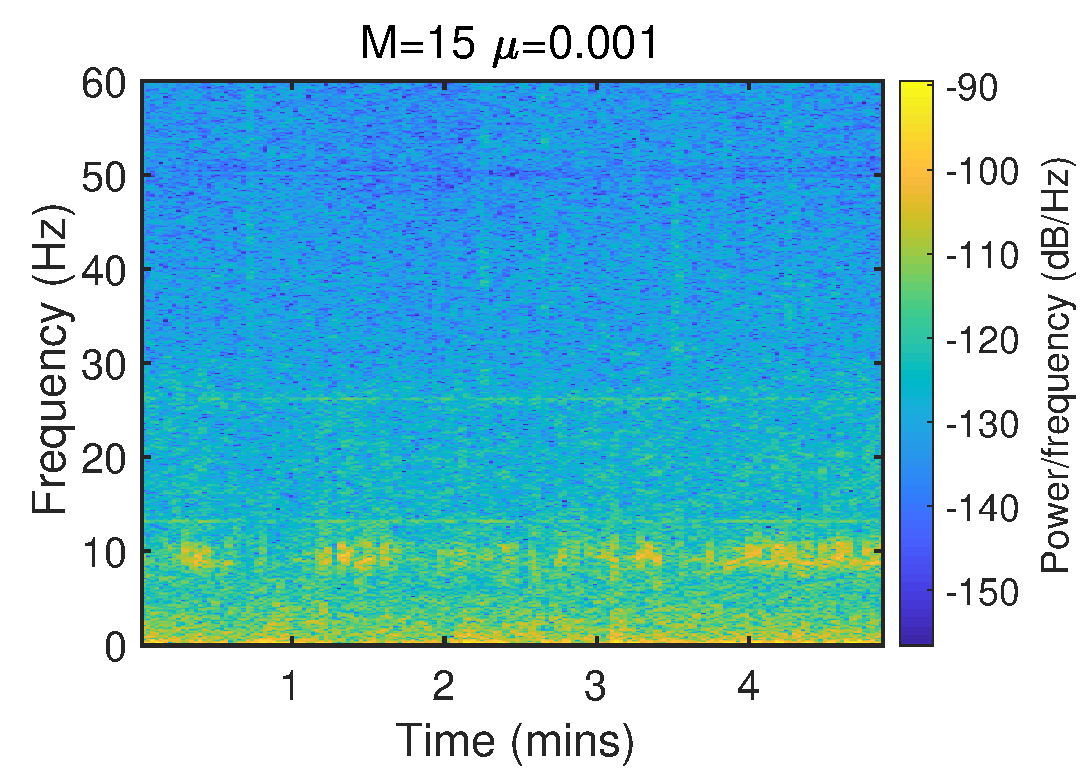
\includegraphics[width=\textwidth]{fig/23/23d8.eps}
    \end{subfigure}
    \hspace{-0.4cm}
    \begin{subfigure}[b]{0.32\textwidth}
     \centering
     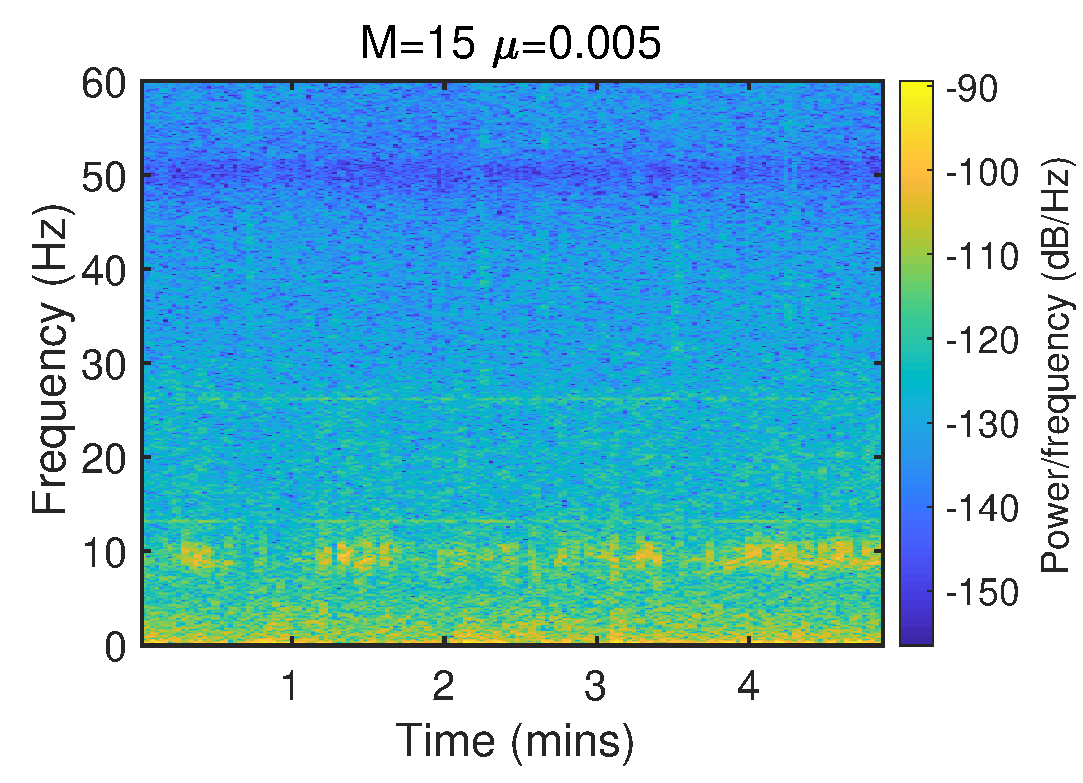
\includegraphics[width=\textwidth]{fig/23/23d9.eps}
    \end{subfigure}
    \hspace{-0.4cm}
    \begin{subfigure}[b]{0.32\textwidth}
     \centering
     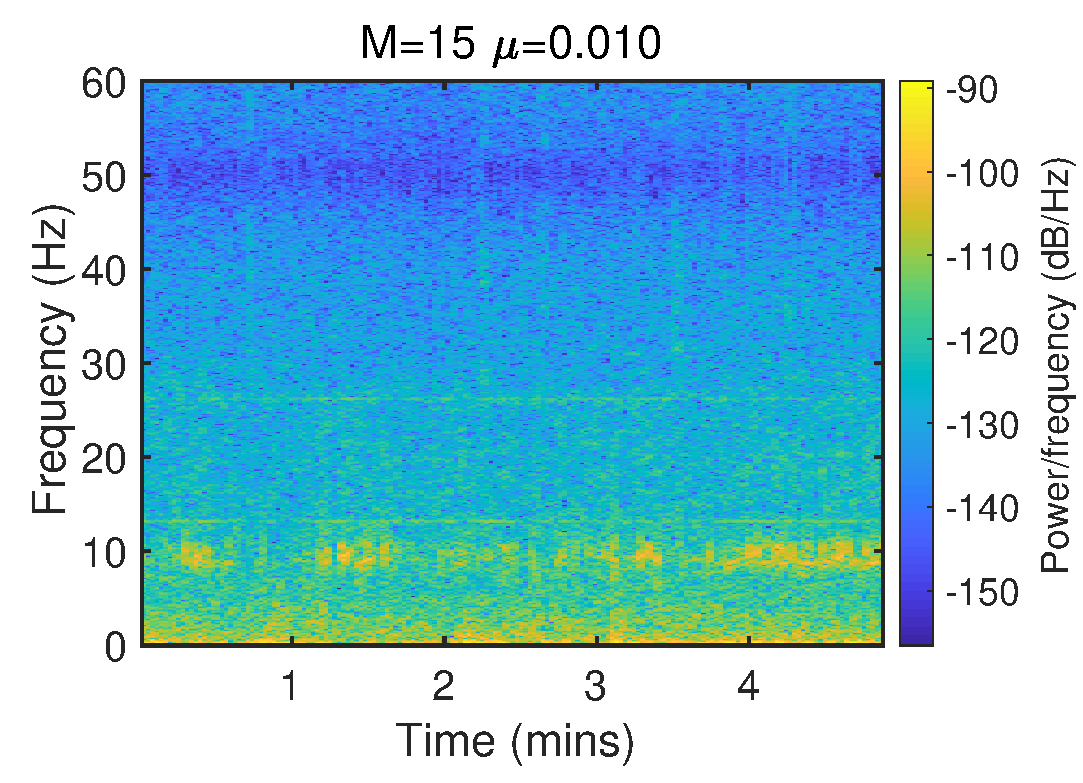
\includegraphics[width=\textwidth]{fig/23/23d10.eps}
    \end{subfigure}
    \caption{ANC POz Spectrogram: Effect of $M$ and $\mu$}
    \label{fig:2_3_d2}
\end{figure}\\
Fig.\ref{fig:2_3_d3} shows the periodograms of original and ANC data at $\mu=0.0001$ and $M=10$. Only the component at $50Hz$ is suppressed and others are nearly same compared with original signal.
\begin{figure}[htb]
    \centering
    \hspace{-0.4cm}
    \begin{subfigure}[b]{0.35\textwidth}
     \centering
     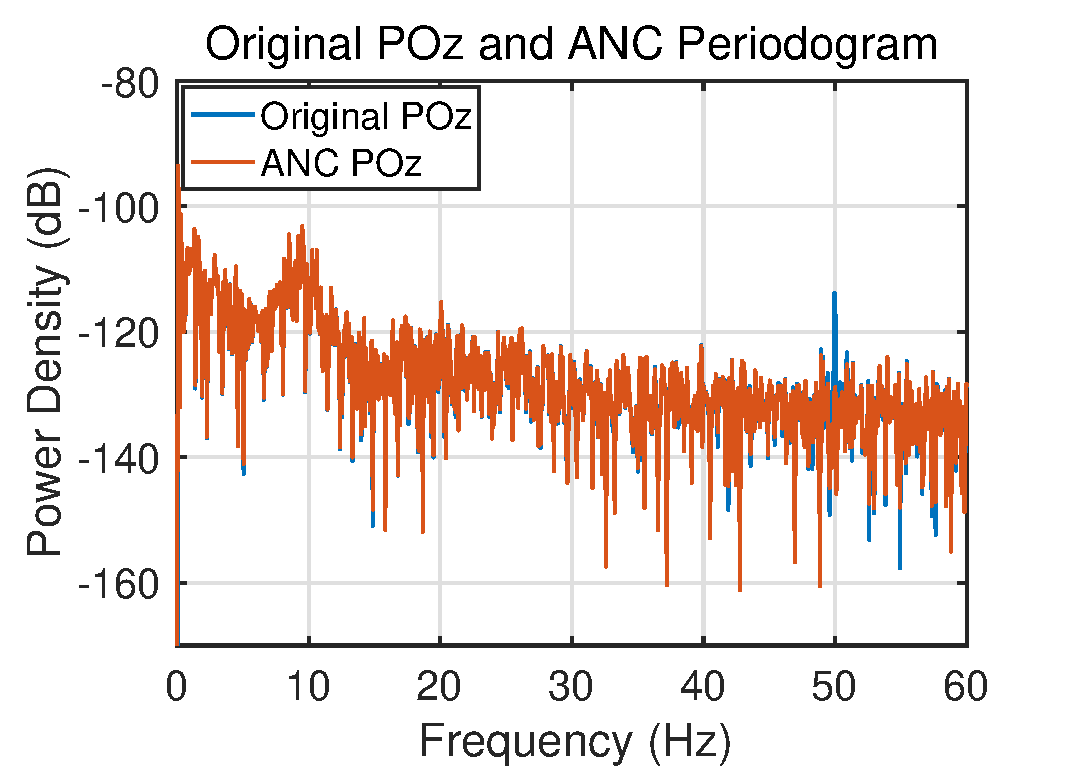
\includegraphics[width=\textwidth]{fig/23/23d11.eps}
    \end{subfigure}
    \hspace{-0.4cm}
    \begin{subfigure}[b]{0.35\textwidth}
     \centering
     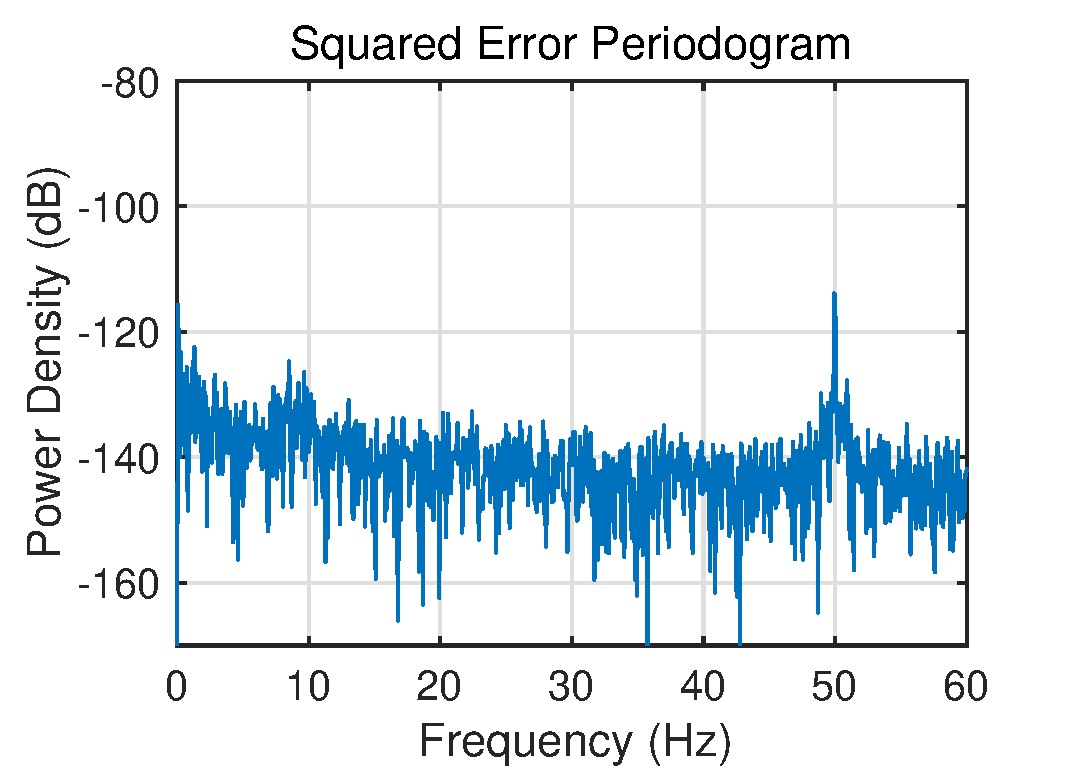
\includegraphics[width=\textwidth]{fig/23/23d12.eps}
    \end{subfigure}  
    \caption{Periodograms and Squared error of Original EEG and de-noising EEG}
    \label{fig:2_3_d3}
\end{figure}



